% INTRODUCTION CHAPTER
\chapter{Introduction}\label{ch:introduction}
\section{Context}\label{sec:Context}
Esports is a form of competition using video games where participants will compete either individually or in a team for a chance at victory.
These competitions attract millions of viewers, with estimates of 532 million spectators by the end of 2022, and this value is expected to grow annually at a value of roughly 8.7\%~\citep{newzoo2022viewers}.
The rapid growth in Esports has led to the industry becoming professional, with hundreds of players contracted on full-time contracts competing for prize pools of up to \$40 million~\citep{esportsearnings}.
According to~\citet{newzoo2022viewers} this viewership will help the industry generate over \$1.38 billion in revenue by the end of 2022.
As the Esports industry continues to grow, so does the importance on teams to win and remain relevant in the industry.\\

In traditional sports, analytics has become an extremely popular field with teams investing heavily in some form of analytics.
These analytics can be used from evaluating opposing teams, to individual player forecasting and even used to decide signings or team selection~\citep{sarlis2020sports, apostolou2019sports}.
\citet{apostolou2019sports, sarlis2020sports} shows that these analytics can be applied for each athlete, giving an accurate estimation of key metrics such as goals scored per season or the number of shots attempted in a given match.
This same methodology could be applied to Esports, using these machine learning techniques could highlight specific factors both pre-game and in-game, helping analysts and coaches refine strategies within the game.\\

The ease of data collection coming from each match has led to a rise in Esports analytics.
In-depth analysis of matches, teams and pre-game factors become key techniques for teams to gain this advantage over their competitors, with teams being required by their leagues to have at least one dedicated coach and analyst similar to traditional sports teams~\citep{LCSRules}.
These coaches and analysts use predictive analytics to maximise their team's likelihood of winning by altering numerous features related to pre-game and in-game strategies, current \gls{meta} analysis and common patterns of their competition~\citep{kokkinakis2021metagaming}.
However, this analysis is often completed manually by watching key highlights of matches using the analyst's intuition and using rudimentary analysis of in-game factors.\\

If matches can be accurately predicted using machine learning techniques, then analysts can provide new opportunities to optimise player strategies and can lead their teams to better outcomes.
Applying the same findings found in~\citet{gray2012customer}, it can be seen that the overall performance and fan satisfaction with a sports team's performance has a measurable impact on revenue via fan attendance and their media response.
Esports fans also appear to increasingly demand skillful performances especially from players that are deemed as \emph{'superstars'}, with these players being more likely to attract new viewers, thus increasing the economic gain of the market~\citep{mangeloja2019economics, ward2019esport}.
It would then be in the interest of both teams and individual players to maximise their abilities and career longevity using these advanced analytics, so they can fully realise their potential;
especially when the volatility of a players job security results in only the top 10\% of players having lasting, stable careers~\citep{ward2019esport}.\\


\section{League of Legends}\label{sec:League of Legends}
\subsection{General Information}\label{subsec:general-information}
League of Legends is a \ac{MOBA} game developed by Riot Games released in 2009, it is one of most popular esports games in the world with over 180 million monthly players and a peak of 73.8 million concurrent viewers~\citep{riotplayercount, upcomerworld2021}.
A \ac{MOBA} is fusion genre of real-time strategy, role-playing and action games in which two sets of teams will compete in a known arena.
The objective of each game is to defeat the opposition by destroying the enemy's base.\\

Each player will select and control a unique~\gls{champion} with their own set of distinct abilities, this~\gls{champion} will be selected before the game starts and cannot be changed until the game has ended - this will be covered further in Section~\ref{subsec:champ-select}.
Players can strengthen their~\glspl{champion} by gaining experience and gold, this can be done by slaying enemy~\glspl{minion}, \gls{jungle} monsters, enemy structures or enemy \glspl{champion}.
This gold can be spent in the shop allowing players to purchase items that enhance the attributes of their \gls{champion}, as well as various utility items such as \glspl{ward}.\\

\begin{figure}[h!]
    \centering
    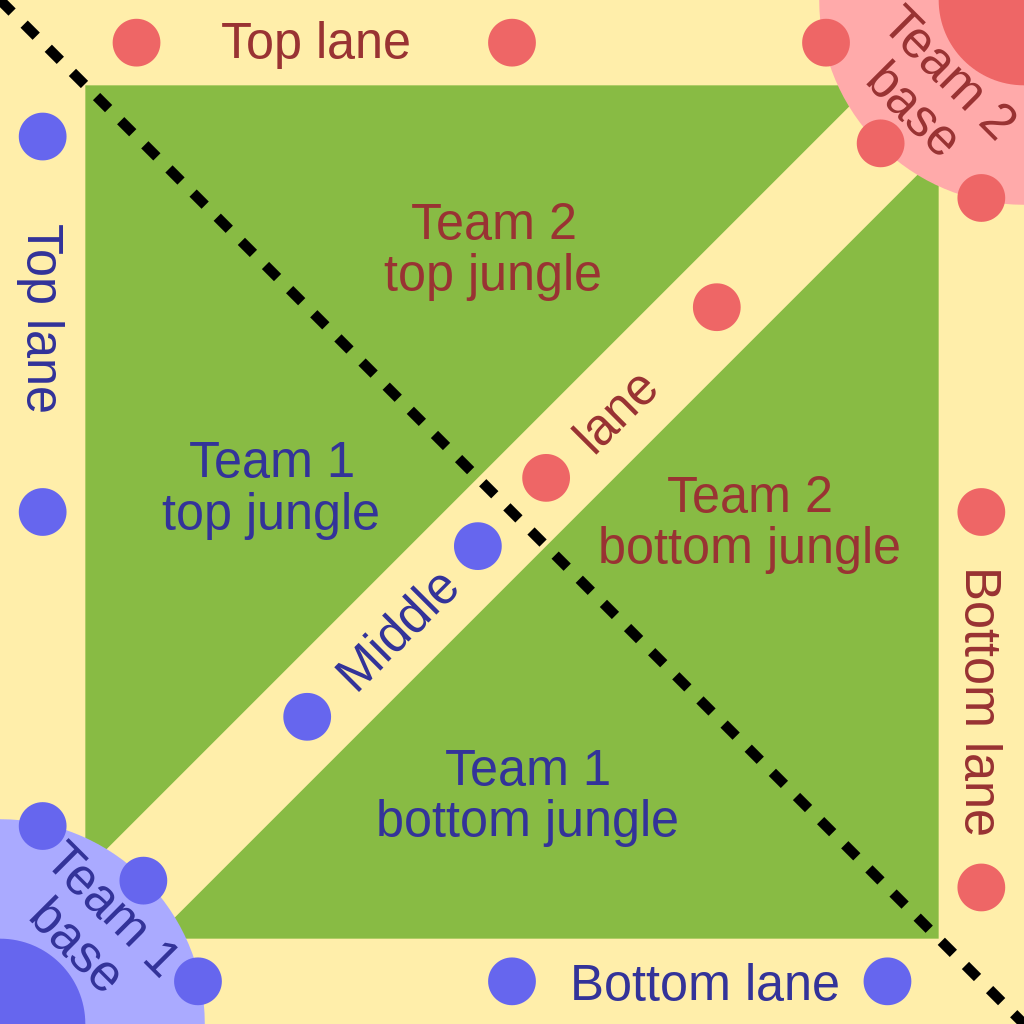
\includegraphics[width=0.5\textwidth]{figures/MOBAMap}
    \caption{Map of League of Legends}
    \label{fig:Lolmap}
\end{figure}

A map of League of Legends can be seen in Figure~\ref{fig:Lolmap}.
There are three lanes, Top, Middle and Bottom, with the \gls{jungle} filling the space between these lanes.
Typically, a player will be assigned to each of these lanes including the jungle, the exception being two players assigned to the bottom lane.
Each coloured dot represents a \gls{tower} that must be taken in order to reach the enemy \Gls{nexus}.
A river separates the territories between the Blue (Team 1) and the Red team (Team 2) along the dotted black line seen in Figure~\ref{fig:Lolmap}.
In this river you can find \Gls{baron} or \Gls{rift herald} in top-side and the \Gls{dragon} in the bottom-side, they are key objectives that will often be contested.

\subsection{Champion Selection}\label{subsec:champ-select}

Champion Selection plays an important part in every game of League of Legends.
Certain champions have inherent synergies with one another, meaning they are beneficial to be picked with each other.
Likewise, some champions are considered counter matchups when they are good at stopping another champion.
This means that picking a good mixture of \glspl{champion} that are solid synergistically, whilst also ensuring the opponents \glspl{champion} do not counter yours is vital.
These ideas are the fundamentals of champion selection, and they are what professional coaches and analysts attempt to solve each week.
Factors such as player champion experience, the current game balance \gls{patch} or a champion's ability to be flexible across different lanes will change champion select from game to game. \\

As seen in Figure~\ref{fig:draft}, the current draft phase works as follows:
\begin{itemize}
    \item Ban Phase 1 begins with the Blue team, in turn each team bans three champions from the pool.
    \item Pick Phase 1 begins with a singular pick from the Blue side, followed by two picks from the Red side.
     Blue side will get two more picks, followed by a singular pick from Red side for three picks each.
    \item It will then enter Ban Phase 2.
    Here both teams will ban two more champions in turn, with Red side starting.
    \item Pick Phase 2 will begin.
    Here Red side get their fourth champion pick, followed by the final two picks from Blue side and finally Red side pick their final champion.
\end{itemize}

\begin{figure}[h!]
    \centering
    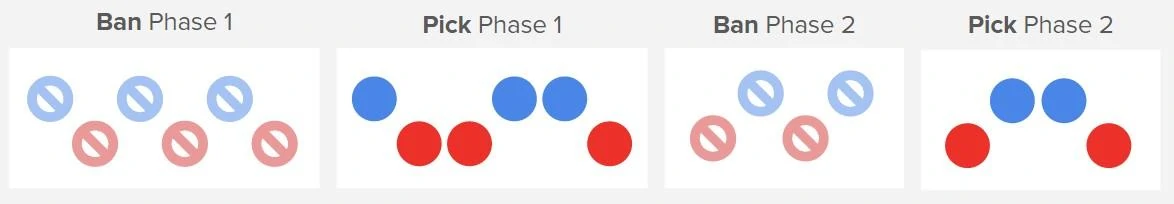
\includegraphics[width=1\textwidth]{figures/DraftPhase}
    \caption{Champion Select}
    \label{fig:draft}
\end{figure}

This champion selection structure leads to clear opportunities for teams to ban out champions that are deemed too strong in Ban Phase 1.
Blue side getting the first pick gives them a chance to pick any champion that is deemed too strong that still remains after Ban Phase 1.
Whilst Red side getting the last pick gives a defined opportunity to pick a counter match-up to any given lane.
These factors can give one side the edge based on the \Gls{patch}, leading to varying strength levels of Blue side vs Red side and can make side selection important.

\section{Structure, Aims, and Objectives}\label{sec:Structure, Aims, and Objectives}

The following section explores an overview of this dissertation:

The next chapter, Chapter~\ref{ch:literaturereview}, discusses the role of...

Chapter~\ref{ch:methodology} follows the techniques and tools used for predicting the effect of pre-game choices on the outcome of the match.
Beginning with...


Chapter~\ref{ch:results} then proceeds with a discussion of the work
carried out and presents the outputs of the model created.
An evaluation of...

Finally, chapter~\ref{ch:conclusion} will conclude the dissertation giving an overall summary of the work completed, as well as any further opportunities for research. \\


Having pre-established the landscape of Esports and its relationship with analytics, it is clear that refinement in the way that this industry uses its highly available data is needed.
Many academics have predicted the outcomes of matches in Esports titles such as ~\citet{silva2018continuous}.
However, performing these studies, few academics addressed the implications of the champion select phase on the overall outcome on a given League of Legends match.
Often it is put into the model as a singular feature defined as champion or ban, without giving much implication on how an individual champion effects a game more than another.
In contrast to other studies, this study uses a much larger, updated dataset and will concentrate much more on the overall effects of the pre-game choices that a team will make inside champion select.
This includes the effects of each individual champion on the likelihood of winning a match.
Therefore, the research question that will be addressed is as follows:

\begin{quote}  \emph{Can the outcome of a League of Legends match be predicted?} \end{quote}


This research will provide an overview of the changing ways in which video games are being consumed, both in the emergence of esports and of the betting activities associated therewith.
Subsequently, this article outlines the hypothesised relationships between demographic characteristics, media consumption practices and esports betting practices before describing the research model employed in this study.
After outlining the methods, measures, participants and procedures this article presents, the results of the study in reference to demographic characteristics and measures of consumption.
The findings are discussed alongside their theoretical and practical implications, potential avenues of future research, and the limitations of this work.

This research will thus contribute to the growing body of literature related to the convergence of gambling and (video) gaming.
Specifically, this study investigates the interrelations between the motivations for consuming esports, consumption of digital media products associated with esports and participation in esports betting.
As such, this work will provide evidence whether esports betting replicates relationships present in traditional sports betting, or if this emergent activity is accompanied by novel relationships.